\documentclass{ctexbeamer}        % 文档类beamer的汉化版本
%\documentclass{beamer}

\usefonttheme{serif}              % 使用衬线字体
\usefonttheme{professionalfonts}  % 数学公式字体

\usepackage{mathtools}
\usepackage{graphicx}
\usepackage{xcolor}
\usepackage{listings}
\usepackage{booktabs}
\usepackage{amsmath}
\usepackage{bm}
\usepackage{svg}
\usepackage[backend=biber]{biblatex}
\bibliography{bibliography.bib}


%% --> 配置中英文字体
% \usepackage{fontspec}
% \setmainfont{Liberation Serif}
% \setsansfont{DejaVu Sans}
% \setmonofont{Cousine}
% \usepackage{xeCJK}
% \setCJKmainfont[BoldFont=Noto Sans SC]{Noto Serif SC}
% \setCJKsansfont{Noto Sans SC}
% \setCJKmonofont{WenQuanYi Micro Hei Mono}

%% --> 主题和色彩风格
\usetheme{Montpellier}
\usecolortheme{beaver}
\definecolor{darkgreen}{rgb}{0.0, 0.2, 0.13}
%\lstset{language=Python,
%        basicstyle=\ttfamily\bfseries,
%        commentstyle=\color{red}\itshape,
%        stringstyle=\color{darkgreen},
%        showstringspaces=false,
%        keywordstyle=\color{blue}\bfseries,
%        basicstyle=\scriptsize,
%        frame=shadowbox}

\beamertemplatenavigationsymbolsempty

\begin{document}
\title{Body Fat Project Presentation}
\author{Group-20}
\date{October 20, 2022}
\frame{\titlepage}


\begin{frame}{Summary of Data Cleaning}

\begin{itemize}
\item We drop the sample whose estimated body fat is negative. The estimated fat is infered from Siri's equation:

$$
\rm Fat=\frac{495}{Density} - 450
$$

The sample's statistics are listed below:
\newline

\begin{tabular}{cccccc}
   \toprule
   IDNO & BODYFAT & DENSITY & Estimated Body Fat\\
   \midrule
   182 & 0.0 & 1.1089 & -3.6117 \\
   \bottomrule
\end{tabular}
\end{itemize}
\end{frame}


\begin{frame}{Summary of Data Cleaning}

\begin{itemize}
\item From the scatter plot of body fat and density, we find there are 3 obvious outliers. We use the Siri's equation to compute the estimated body fat and substract it by corresponding the original BODYFAT to get errors.

\begin{figure}
   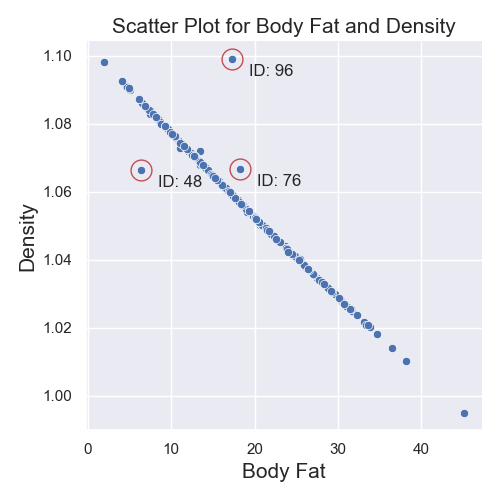
\includegraphics[width=0.425\textwidth]{../image/scatter_plot_for_density_and_fat.png}
   \hfill
   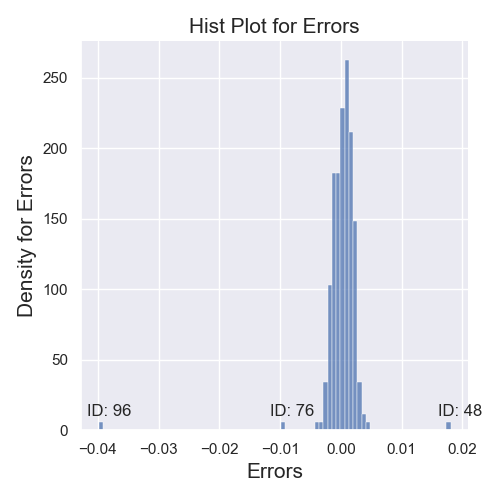
\includegraphics[width=0.425\textwidth]{../image/hist_plot_for_errors.png}
\end{figure}
\end{itemize}

\end{frame}


\begin{frame}{Summary of Data Cleaning}

\begin{itemize}
\item We use $3-\sigma$ criterion on the errors to find out these outliers. Finally, we use estimated body fat from Siri's equation to replace the original body fat for these samples.
\newline

\begin{tabular}{cccccc}
   \toprule
   IDNO & BODYFAT & Estimated Body Fat & Error\\
   \midrule
   48 & 6.4 & 14.1350 & 7.7350 \\
   76 & 18.3 & 14.0915 & -4.2085 \\   
   96 & 17.3 & 0.3685 & -16.9315 \\
   \bottomrule
\end{tabular}
\end{itemize}

\end{frame}

\end{document}